\documentclass[../Head/Main.tex]{subfiles}
\begin{document}
\subsection{Environment}
\label{subsec:design_environment}
The two-wheeled robot should navigate around the environment called “bigworld” shown on figure \ref{fig:bigworld_white}. To do so, it have been chosen to divide the environment into rooms. The natural definition of \textit{'rooms'} have been taken into account, resulting in a 14 room layout. This can be seen on figure \ref{fig:bigworld_14_rooms}, where each room can be distinguished by different grey scale colours. 

\begin{figure}[H]
	\centering
	\begin{subfigure}[b]{0.49\textwidth}
		\centering
		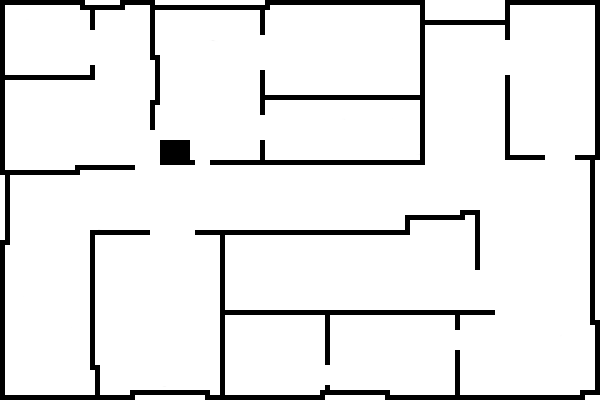
\includegraphics[width=\textwidth]{map_medium_white}
		\caption{Illustration of the world "bigworld"}
		\label{fig:bigworld_white}
	\end{subfigure}
	\hfill	
	\begin{subfigure}[b]{0.49\textwidth}
		\centering
		\begin{tikzpicture}
		\node[anchor=south west, inner sep=0] (image) at (0,0) {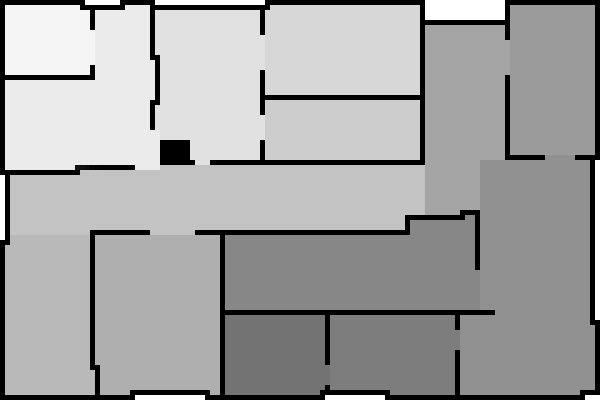
\includegraphics[width=\textwidth]{map_medium}};
		\node[align=center, black, font={\small}] at (0.7,5) {Room 1};
		\node[align=center, black, font={\small}] at (1.2,3.9) {Room 2};
		\node[align=center, black, font={\small}] at (2.9,4.5) {Room 3};
		\node[align=center, black, font={\small}] at (4.75,4.9) {Room 4};
		\node[align=center, black, font={\small}] at (4.76,3.75) {Room 5};
		\node[align=center, black, font={\small}] at (3,2.75) {Room 6};
		\node[align=center, black, font={\small}] at (0.65,1.25) {Room 7};
		\node[align=center, black, font={\small}] at (2.2,1.25) {Room 8};
		\node[align=center, black, font={\small}] at (6.45,4.25) {Room 9};
		\node[align=center, black, font={\small}] at (7.7,4.5) {Room 10};
		\node[align=center, black, font={\small}] at (7.5,1.75) {Room 11};
		\node[align=center, black, font={\small}] at (4.75,1.8) {Room 12};
		\node[align=center, black, font={\small}] at (5.45,0.6) {Room 13};
		\node[align=center, black, font={\small}] at (3.8,0.6) {Room 14};
		\end{tikzpicture}		
		\caption{"bigworld" divided into 14 rooms}
		\label{fig:bigworld_14_rooms}
	\end{subfigure}
	\caption{Illustration of the world "bigworld" before and after it has been divided into 14 rooms}
	\label{fig:bigworld}
\end{figure}
The division into rooms are useful in terms of knowing which rooms that have been searched and which that not yet have been searched for marbles.\\
It is also useful as an abstract state space for reinforcement learning such that it can be found which order the rooms  should be visited.


\end{document}